\def\pgfsysdriver{pgfsys-dvisvgm.def}
\documentclass[tikz,border=8pt]{standalone}
\usepackage{amsmath}
% Semantic palette shared by the light and dark exports; geometry and TeX glyphs stay identical.
\ifdefined\FigureDark
  \definecolor{FigureForeground}{HTML}{E1E8DF}
  \definecolor{FigureMuted}{HTML}{94A69B}
  \definecolor{FigureBlue}{HTML}{8CC5F2}
  \definecolor{FigureOrange}{HTML}{F4B76B}
  \definecolor{FigureRed}{HTML}{F28E86}
  \definecolor{FigureBlueFill}{HTML}{273F4F}
  \definecolor{FigureOrangeFill}{HTML}{4A3726}
  \definecolor{FigurePaper}{HTML}{1B2420}
\else
  \definecolor{FigureForeground}{HTML}{202C29}
  \definecolor{FigureMuted}{HTML}{68766E}
  \definecolor{FigureBlue}{HTML}{245A88}
  \definecolor{FigureOrange}{HTML}{986000}
  \definecolor{FigureRed}{HTML}{A44030}
  \definecolor{FigureBlueFill}{HTML}{E5EDF8}
  \definecolor{FigureOrangeFill}{HTML}{FFF0D8}
  \definecolor{FigurePaper}{HTML}{FBFAF7}
\fi

% Face luminance preserves the same upper-right lighting in both reader themes.
\ifdefined\FigureDark
  \definecolor{CubeTop}{HTML}{46677F}
  \definecolor{CubeRight}{HTML}{304B60}
  \definecolor{CubeLeft}{HTML}{243747}
\else
  \definecolor{CubeTop}{HTML}{EDF3FC}
  \definecolor{CubeRight}{HTML}{CADCEC}
  \definecolor{CubeLeft}{HTML}{8FABCB}
\fi
\begin{document}
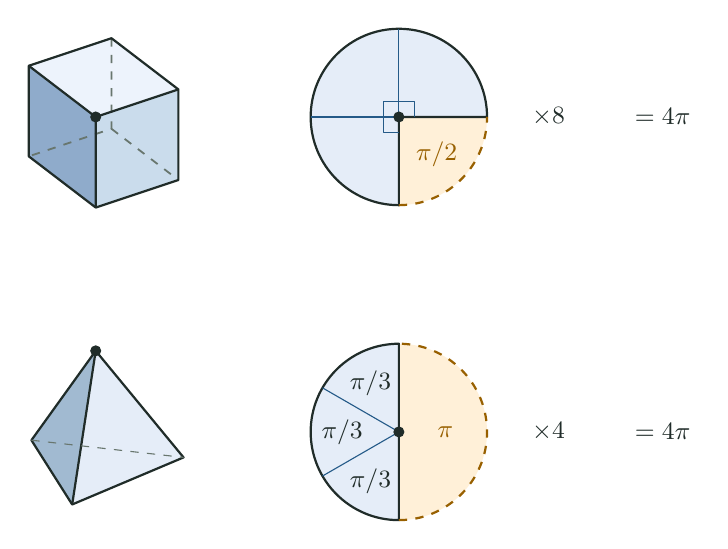
\begin{tikzpicture}[color=FigureForeground,>=stealth,
  every node/.style={font=\small},line join=round]
% Original composition: cube above tetrahedron; each row reads left to right.
\def\SecondX{0}\def\SecondY{-4}
% The left panels are projections: face-angle values belong only to the
% intrinsic planar fans on the right. Each dot selects their common vertex.
\begin{scope}

\begin{scope}[shift={(1.05,.05)}]
% Projected cube basis vectors (1.05,.35), (-.85,.65), (0,-1.15).
% The three visible quadrilaterals share O; their union has six outer edges.
\coordinate (O) at (0,0);
\coordinate (A) at (1.05,.35);
\coordinate (B) at (-.85,.65);
\coordinate (C) at (0,-1.15);
\coordinate (AB) at (.20,1.00);
\coordinate (BC) at (-.85,-.50);
\coordinate (CA) at (1.05,-.80);
\coordinate (ABC) at (.20,-.15);
\fill[CubeTop] (O)--(A)--(AB)--(B)--cycle;
\fill[CubeLeft] (O)--(B)--(BC)--(C)--cycle;
\fill[CubeRight] (O)--(C)--(CA)--(A)--cycle;
% The opposite corner is A+B+C. Its three incident edges are occluded.
\draw[dashed,line width=.65pt,FigureMuted] (AB)--(ABC)--(BC) (ABC)--(CA);
\draw[thick] (A)--(AB)--(B)--(BC)--(C)--(CA)--cycle;
\draw[thick] (O)--(A) (O)--(B) (O)--(C);
\fill (O) circle (2pt);
\end{scope}
\begin{scope}[shift={(4.90,.05)}]
\fill[FigureBlueFill] (0,0)--(1.12,0) arc (0:270:1.12)--cycle;
\fill[FigureOrangeFill] (0,0)--(0,-1.12) arc (270:360:1.12)--cycle;
\draw[thick] (0,0)--(1.12,0) arc (0:270:1.12)--cycle;
\draw[FigureBlue] (0,0)--(0,1.12) (0,0)--(-1.12,0);
\draw[dashed,thick,FigureOrange] (0,-1.12) arc (270:360:1.12);
\fill (0,0) circle (2pt);
% Intrinsic right-angle marks replace repeated numeric labels.
\draw[FigureBlue] (.20,0)--(.20,.20)--(0,.20);
\draw[FigureBlue] (0,.20)--(-.20,.20)--(-.20,0);
\draw[FigureBlue] (-.20,0)--(-.20,-.20)--(0,-.20);
\node[FigureOrange] at (.48,-.48) {$\pi/2$};
\end{scope}
% Arithmetic occupies the same row as the local deficit, as in the original.
\node at (6.80,.05) {$\times 8$};
\node at (8.25,.05) {$=4\pi$};
\end{scope}
\begin{scope}[shift={(\SecondX,\SecondY)}]

\begin{scope}[shift={(1.05,.05)}]
% Orthographic view of a regular tetrahedron: azimuth 15 deg, elevation 25 deg.
% Three-dimensional vertices before projection:
% O=(0,0,sqrt(8/3)), A=(-1,-1/sqrt(3),0),
% B=(1,-1/sqrt(3),0), C=(0,2/sqrt(3),0).
% screen x=cos(15)x-sin(15)y;
% screen y=cos(25)z-sin(25)(sin(15)x+cos(15)y)-0.45.
\coordinate (O) at (0,1.0300);
\coordinate (A) at (-.8165,-.1049);
\coordinate (B) at (1.1154,-.3237);
\coordinate (C) at (-.2989,-.9214);
\fill[FigureBlueFill!65!FigureBlue] (O)--(A)--(C)--cycle;
\fill[FigureBlueFill] (O)--(C)--(B)--cycle;
\draw[thick] (O)--(A)--(C)--(B)--cycle;
\draw[thick] (O)--(C);
\draw[dashed,FigureMuted] (A)--(B);
\fill (O) circle (2pt);
\end{scope}
\begin{scope}[shift={(4.90,.05)}]
\fill[FigureBlueFill] (0,0)--(0,1.12) arc (90:270:1.12)--cycle;
\fill[FigureOrangeFill] (0,0)--(0,-1.12) arc (270:450:1.12)--cycle;
\draw[thick] (0,1.12) arc (90:270:1.12)--cycle;
\draw[FigureBlue] (0,0)--(150:1.12) (0,0)--(210:1.12);
\draw[dashed,thick,FigureOrange] (0,-1.12) arc (270:450:1.12);
\fill (0,0) circle (2pt);
\node at (120:.72) {$\pi/3$};
\node at (180:.72) {$\pi/3$};
\node at (240:.72) {$\pi/3$};
\node[FigureOrange] at (.59,0) {$\pi$};
\end{scope}
\node at (6.80,.05) {$\times 4$};
\node at (8.25,.05) {$=4\pi$};
\end{scope}
\end{tikzpicture}
\end{document}
